\documentclass[a4paper]{article}

\usepackage{parskip}
\usepackage{enumitem}
\usepackage{graphicx}
\usepackage{multicol}
\usepackage[colorlinks=true]{hyperref}

\usepackage{geometry}
\usepackage[paper=portrait,pagesize]{typearea}

\setitemize{noitemsep,topsep=0pt,parsep=0pt,partopsep=0pt}


\title{Voorstel Studieprogramma Bachelor Informatica}
\author{Joey De Pauw}
\date{}



\newcommand*{\includeFullPage}[1]{ %
    \newpage%
    \vspace*{-2.5cm}%
    \hspace*{-0.16\textwidth}%
    \includegraphics[width=1.34\textwidth]{{ '{#1}' }}%
}


\begin{document}

    \maketitle

    \section{Introductie}

        Onze bacheloropleiding bestaat uit 180 studiepunten verdeeld over verschillende vakken. Deze vakken zijn natuurlijk een dynamisch gegeven en doorheen de jaren wordt niet enkel de inhoud ge\"updatet, maar ook de evaluatievormen en volgtijdelijkheden. Dit gebeurt typisch nogal ad hoc per prof per cursus, wat het natuurlijk moeilijk maakt om ook globaal een gebalanceerd studieprogramma met gestroomlijnde volgtijdelijkheid te bekomen.

        Hier komen de studenten aan te pas. Als studentenvertegenwoordiger en ex-bachelor student heb ik samen met andere studenten (Ba en Ma) ons huidige studieprogramma grondig bestudeerd. Uit deze studie en enkele getuigenissen van onze studenten blijkt dat er twee grote problemen zitten in ons studieprogramma:
            - Het eerste semester van het 3de jaar wordt veel zwaarder ervaren dan alle andere semesters. Anderzijds wordt opgemerkt dat de werklast in het 2de jaar relatief laag is.
            - Sommige vakken hebben disproportioneel veel volgtijdelijkheden in verhouding met het aantal studiepunten. Te restrictief zijn kan een probleem vormen voor de doorstroom.

        Gelukkig kunnen beide problemen opgelost worden door het herzien van de volgtijdelijkheden en het herverdelen van het studieprogramma. Ik stel een vernieuwd studieprogramma voor met minimale wijzigingen en een zo klein mogelijke impact voor zowel de studenten als de lesgevers.

        Dit voorstel werd bekomen door voor elk vak de volgtijdelijkheid te bekijken met het volgende idee: "Welke kennis is essentieel nodig om aan dit vak te kunnen beginnen?" Er werd dus geen rekening gehouden met subjectieve factoren als de moeilijkheidsgraad van de vakken ("Als een student van A niet kan, zal hij/zij vak B ook niet kunnen.")

        Voor elk vak waar een wijziging in gebeurd is, werd een overzicht gegenereerd met eerst de huidige situatie, vervolgens de wijzigingen relatief en absoluut (met en zonder kleurcode) en ten slotte een legende. De visualisatie geeft de drie bachelorjaren weer met de vakken per semester opgedeeld. Meer details kan u terugvinden in de legende. (Zie Appendix~\ref{sec:appenix}.)

        In sectie~\ref{sec:kleine_wijzigingen} worden de kleine wijzigingen opgelijst. Sectie~\ref{sec:grote_wijzigingen} geeft de grote wijzigingen met bijhorende verklaringen. Ten slotte wordt in sectie~\ref{sec:simulatie} een simulatie toegelicht.

    \newpage
    \newgeometry{left=2cm,right=2cm}
    \section{Kleine Wijzigingen}
    \label{sec:kleine_wijzigingen}

    \begin{multicols*}{2}
        De volgende kleine wijzigingen worden voorgesteld.
        \begin{description}
        
            \pagebreak[3]
            \item[{{ course.name | replace('&','\&') }}] \hfill
            \begin{itemize}
            
                    \item {{ change | replace('&','\&') }}
            
            \end{itemize}
        
        \end{description}
    \end{multicols*}

    \restoregeometry

    \newpage
    \section{Grote Wijzigingen}
    \label{sec:grote_wijzigingen}

    Het voorstel bevat ook enkele grotere algemene wijzigingen. De impact van deze wijzigingen is echter minimaal en wordt in detail besproken:
    \begin{description}[style=nextline]
        \item[\parbox{\linewidth}{DSGA van Ba 3 semester 2 naar Ba 3 semester 1 verplaatst en \\ US van Ba 2 semester 1 naar Ba 2 semester 2 verplaatst.}]
        Dit betreft twee semesterwijziging binnen hetzelfde jaar. Er moet geen overgangsmaatregel zijn. De twee inverse verplaatsingen compenseren deels de impact in werklast voor de lesgever.

        \item[CB van Keuzevakken 2 naar Keuzevakken 1 verplaatst.]
            Dit betreft een semesterwijziging binnen hetzelfde jaar. Er moet geen overgangsmaatregel zijn.

        \item[WP van Ba 3 semester 1 naar Ba 3 semester 2 verplaatst.]
            Dit betreft een semesterwijziging binnen hetzelfde jaar. Er moet geen overgangsmaatregel zijn.

        \item[AI van Ba 3 semester 1 naar Ba 2 semester 1 verplaatst.]
            Jaarwijziging, maar geen semesterwijziging. 2de bachelor studenten kunnen hun oorspronkelijke studieprogramma volgen en AI opnemen in hun derde jaar. 1ste bachelor studenten nemen AI op in hun 2de jaar. Dit heeft als effect dat er 1 overgangsjaar is met meer studenten.

        \item[A\&C van Ba 2 semester 2 naar Ba 3 semester 1 verplaatst.]
            Jaar- EN semesterwijziging. Als het vak naar voor werd geplaatst, zou het twee keer gegeven moeten worden. In dit geval wordt het vak gelukkig naar Ba3 gepusht waardoor er 1 overgangsjaar is met minder/geen studenten.
    \end{description}

    Naast deze 6 verplaatsingen werden er in totaal 16 dependencies verwijderd, 10 toegevoegd en 2 verzwakt. Dit zijn slechts 6 dependencies minder. De volgende punten werden behouden/verbeterd ten opzichte van de huidige situatie:
    \begin{itemize}
        \item Voldoende moeilijke vakken vooraan in studieprogramma om toe te staan dat studenten vroeg ontdekken dat de studie te moeilijk is voor hun.
        \item Voldoende speling voor de studenten om de bacheloropleiding te kunnen spreiden (een jaar met minder dan 36 studiepunten is onder gevuld, maar 150SP van de bachelor moeten behaald zijn om te mogen combineren met de master).
        \item Betere balans tussen de semesters.
        \item Betere balans in werklast over de jaren en semesters.
        \item Voldoende volgtijdelijkheden om te voorkomen dat studenten moeilijke vakken kunnen “laten liggen” tot het einde van hun opleiding. (Dit mitigeert grotendeels de potentieel negatieve gevolgen van de nieuwe regel dat vakken niet meer verplicht opnieuw moeten opgenomen worden.)
    \end{itemize}

    \section{Simulatie}
    \label{sec:simulatie}

    Om deze aanzienlijke verbetering te staven, heb ik een simulatie uitgevoerd waar de gevolgen van 2, 3 of 4 vakken falen berekend worden. Hieruit blijkt dat de volgtijdelijkheid veel beter gebalanceerd is in het voorstel. De voornaamste redenen hiervoor zijn minder bottlenecks en een betere doorstroom omdat studenten niet overdreven afgestraft worden voor het maken van een fout in hun eerste jaar). De details van deze simulatie is te vinden in het bijgevoegde document "simulatie".

    \appendix
    \section{Appendix}
    \label{sec:appenix}

    De appendix bevat visuele representaties van het studieprogramma. De eerste twee figuren geven respectievelijk de huidige situatie en het voorstel weer (relatief ten opzichte van het huidige studieprogramma). Vervolgens wordt de visualisatie getoond per vak om de lijnen makkelijker traceerbaar te maken. Als laatste werd een legende bijgevoegd. Het wordt aangeraden om dit document in fullscreen (F5) te bekijken waardoor de verschillende visualisaties als een animatie werken.

    \pagenumbering{gobble}
    \centering

    \newpage
    \KOMAoptions{paper=landscape,pagesize}
    \recalctypearea

    \includeFullPage{current.pdf}

    \includeFullPage{solution_rel.pdf}

    
        \includeFullPage{Overview/{{ course.id }}_solution_rel.pdf}

    

    \includeFullPage{solution_abs.pdf}

    \newpage
    \KOMAoptions{paper=portrait,pagesize}
    \recalctypearea

    \newpage
    \vspace*{-3.5cm}
    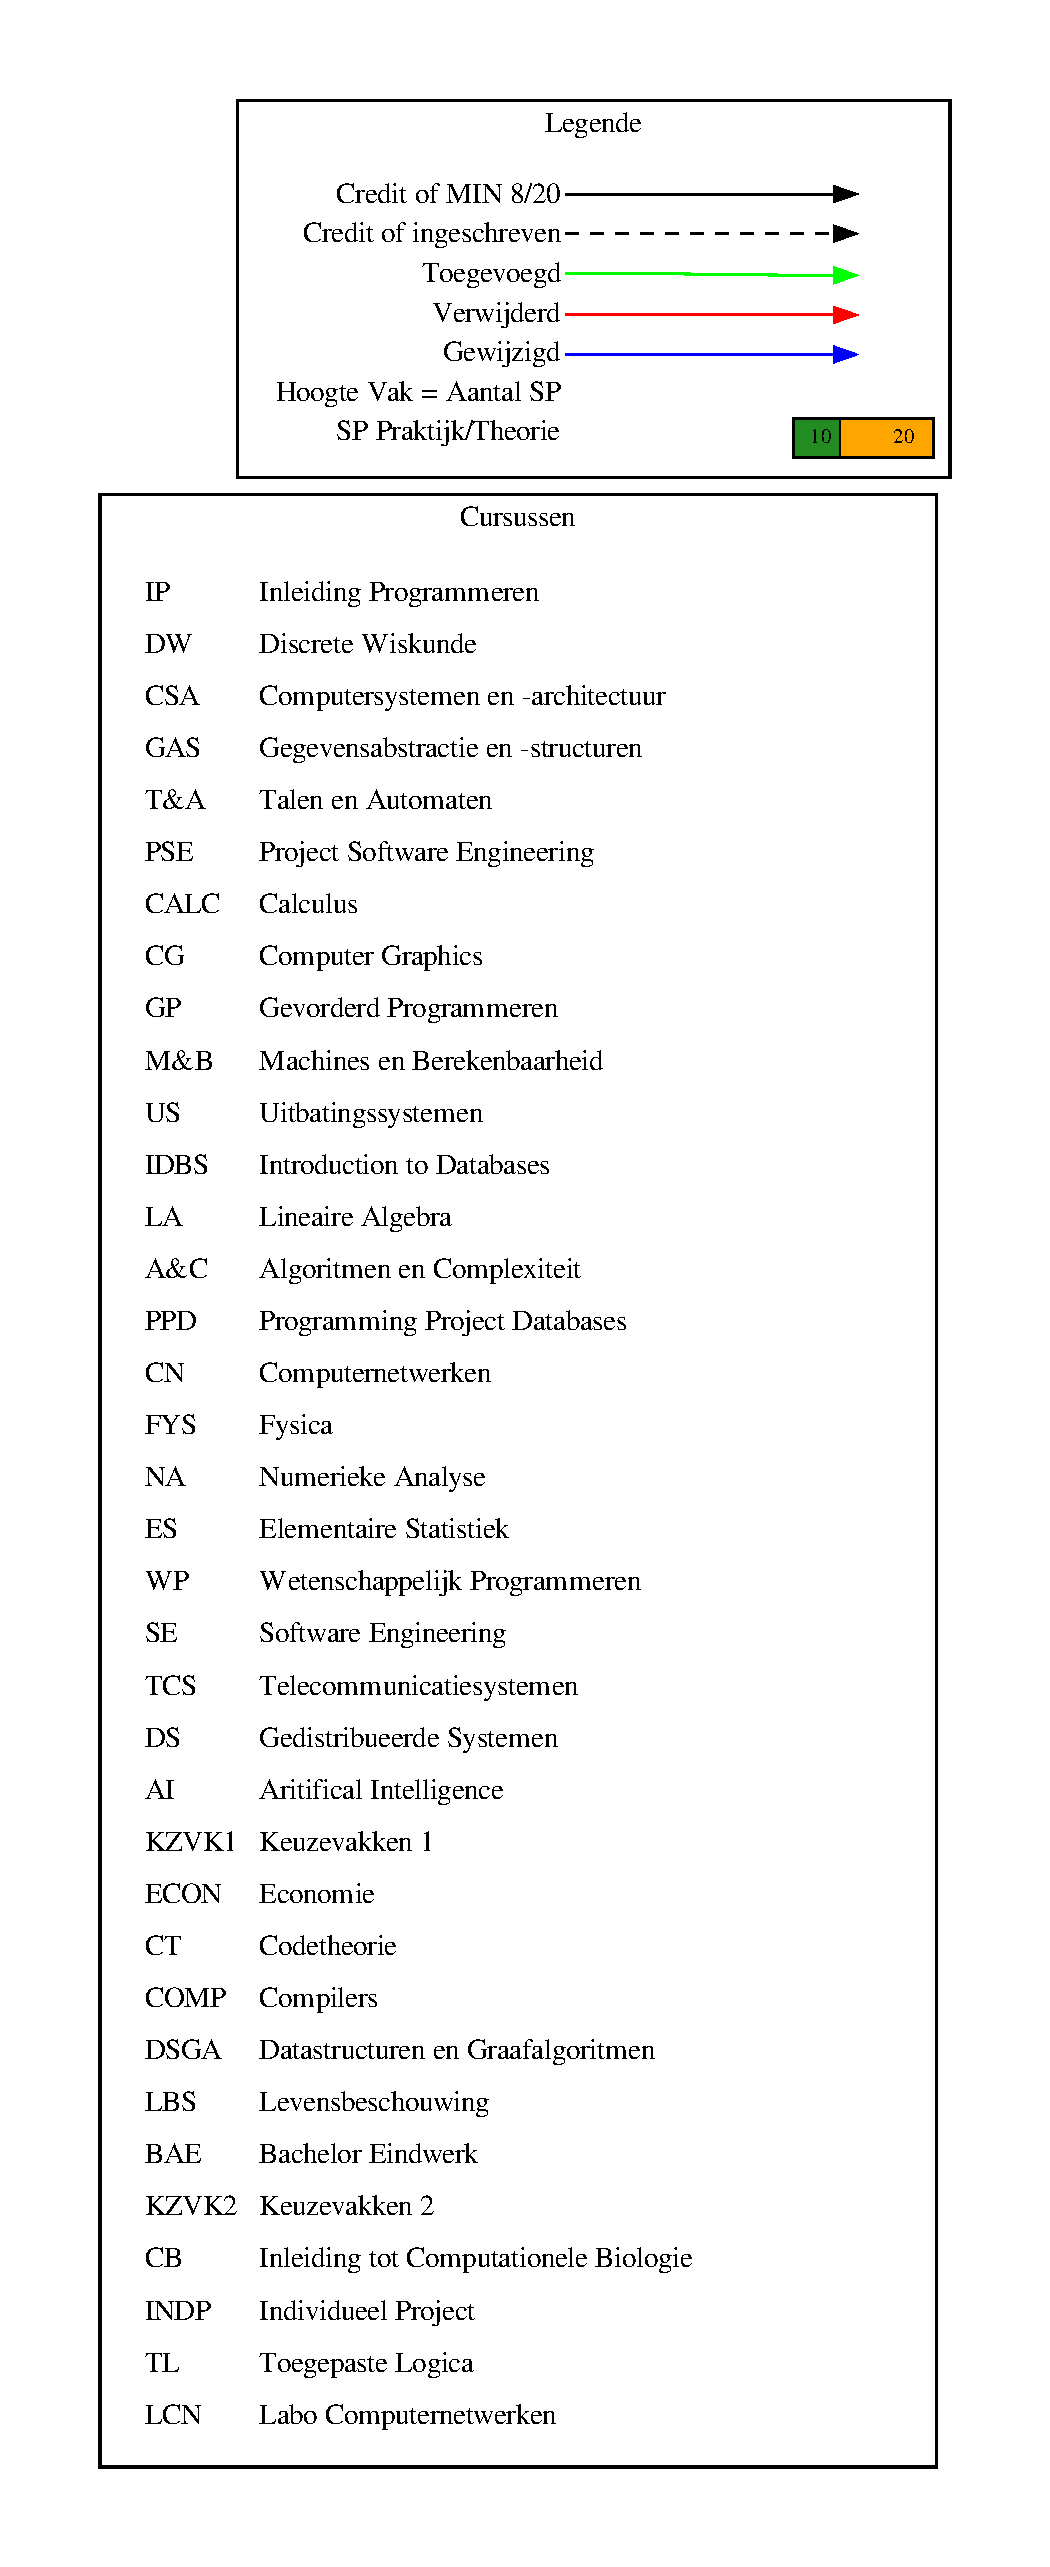
\includegraphics[height=1.5\textheight]{legend.pdf}

\end{document}
